% Experiments. Numbers are from the RTX 4090 run (results/*.csv), multi-seed.
\subsection{Setup}
We simulate $K{=}60$ sensors uniformly placed in a square field (side length
varied from $5$ to $20$~km), a swarm of $M$ rotary-wing UAVs cruising at
$V{=}12$~m/s at altitude $H{=}100$~m, and a battery of about $67$~Wh with a
$15\%$ reserve. The charge time per port is $\tau_{\mathrm{charge}}{=}8$~min. The
propulsion power follows the rotary-wing model \cite{zeng2019energy}, and the
air-to-ground link uses a line-of-sight free-space rate. Candidate stations lie
on a $3{\times}3$ grid; unless stated otherwise the budget is $S_{\max}{=}2$
open stations and $C_{\mathrm{tot}}{=}4$ ports. Every reported value is a mean
over $20$ to $30$ random sensor fields (fixed seeds), with the standard
deviation shown where relevant. All trajectory optimization runs on an
NVIDIA RTX~4090.

\subsection{Queue-model validation against a discrete-event simulation}
The whole analysis rests on the charging-queue model, so we first validate it.
We built a discrete-event simulation (DES) of the actual cycling UAVs, with a
first-in-first-served station and $c$ ports, in which each UAV alternates between
patrolling for a randomized operating time and traveling to the station to
recharge. The simulation supports both exponential and near-deterministic
operating and service times, and we run each configuration over eight seeds and
a long horizon after a warm-up, then measure the true mean queue wait.
Fig.~\ref{fig:des} compares three predictions against the DES. Under
matched assumptions (exponential operating and service), the finite-source
$M/M/c//N$ formula matches the DES to a mean relative error of $4.2\%$, which
confirms the formula. For the realistic system (near-deterministic operating and
charging), the DES wait is lower, so the finite-source model is a
\emph{conservative upper bound} (it exceeds the real wait in $23/23$
configurations). In contrast, the open $M/M/c$ queue overpredicts the DES wait
by about $6\times$ (a mean factor of $5.6$), because it ignores the closed
population: only $M$ UAVs
exist, so the arrival rate falls as more of them are already charging. Using the
open queue therefore distorts the design decisions (we show below that it
produces a spurious placement crossover), which is why we adopt the
finite-source model throughout.

\begin{figure}[t]
  \centering
  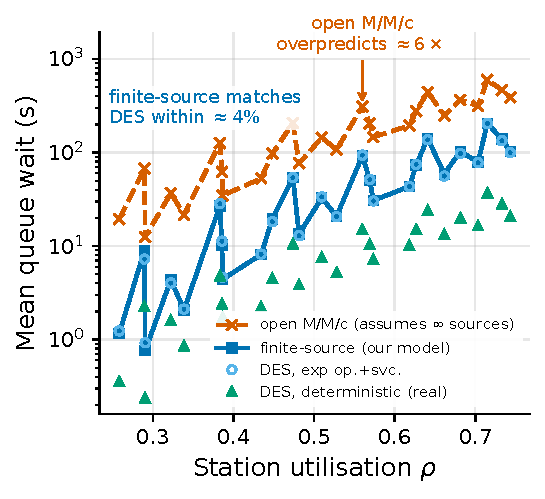
\includegraphics[width=\columnwidth]{../results/fig_des_validation.png}
  \caption{Queue-model validation against discrete-event simulation. The
  finite-source model matches the DES under matched (exponential) assumptions
  and is a conservative upper bound for the real near-deterministic system,
  whereas the open $M/M/c$ overpredicts the wait about $6\times$.}
  \label{fig:des}
\end{figure}

\subsection{Proposition 1: congestion threshold and provisioning}
Fig.~\ref{fig:prop1} plots the peak AoI against swarm size $M$ for several port
budgets. Each curve is U-shaped: increasing $M$ first lowers AoI (denser
coverage) and then raises it (charging congestion), confirming the congestion
threshold of Proposition~\ref{prop:ushape}. The optimal swarm size $M^\star$
grows with the charging capacity, as summarized in Table~\ref{tab:mstar}, which
is exactly the provisioning law: more ports support a larger cost-effective
swarm.

\begin{figure}[t]
  \centering
  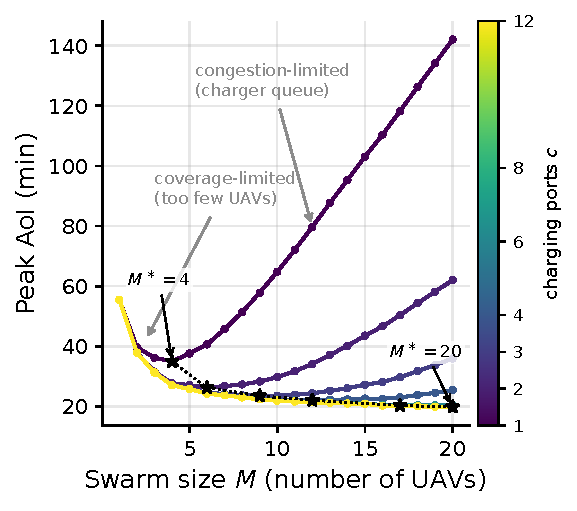
\includegraphics[width=\columnwidth]{../results/fig_prop1_phys.png}
  \caption{Peak AoI is non-monotone in the swarm size $M$ (finite-source model).
  Each port budget has an interior optimal swarm size $M^\star$ (black markers).}
  \label{fig:prop1}
\end{figure}

\begin{table}[t]
  \centering
  \caption{Provisioning law: optimal swarm size $M^\star$ versus port budget $c$.}
  \label{tab:mstar}
  \begin{tabular}{lccccccc}
    \toprule
    Ports $c$        & 1 & 2 & 3 & 4 & 6 & 8 & 12 \\
    \midrule
    $M^\star$        & 4 & 6 & 9 & 12 & 17 & 20 & 20 \\
    \bottomrule
  \end{tabular}
\end{table}

\begin{figure}[t]
  \centering
  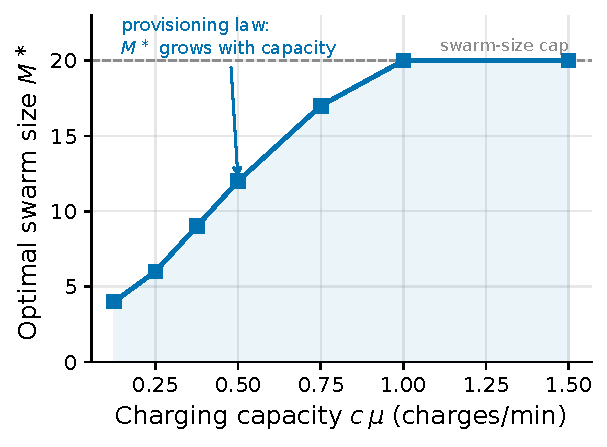
\includegraphics[width=0.86\columnwidth]{../results/fig_prop1_mstar.png}
  \caption{Provisioning law: the optimal swarm size $M^\star$ increases with the
  charging capacity, so a larger port budget supports a larger cost-effective
  swarm.}
  \label{fig:mstar}
\end{figure}

\subsection{Proposition 2: placement inversion}
We compare, per instance, the coverage-optimal placement (minimum recharge
detour, contention-blind) against the traffic-optimal placement (which balances
the queueing load). The traffic-optimal placement lowers the peak AoI in
$19/20$ instances and never increases it, by $14.8\%$ on average, and it selects
\emph{different} station sites in $18/20$ instances (Fig.~\ref{fig:prop2}). This confirms
Proposition~\ref{prop:inversion}: under contention the AoI-optimal placement
inverts from coverage-driven to traffic-driven.

\begin{figure}[t]
  \centering
  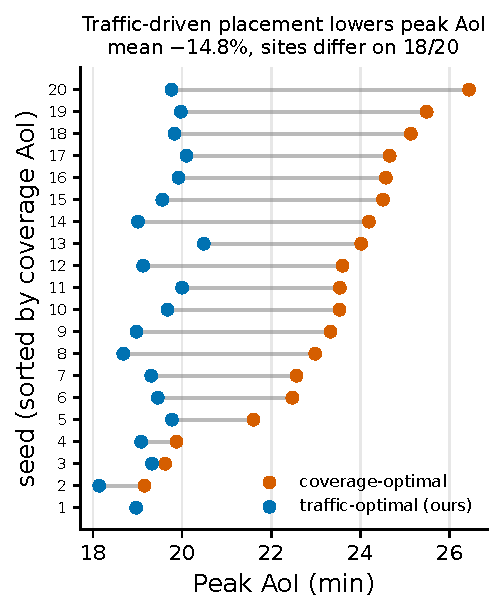
\includegraphics[width=\columnwidth]{../results/fig_prop2.png}
  \caption{Placement inversion. Traffic-optimal placement (which balances the
  queueing load) beats the coverage-optimal (minimum-detour) placement on every
  seed, and chooses different sites on $18/20$ seeds.}
  \label{fig:prop2}
\end{figure}

\subsection{Joint solver versus baselines}
We compare the proposed joint solver (CETSP trajectory with traffic-optimal
placement) against: a single pooled station (all ports at one central station,
the strong Wei-style baseline \cite{wei2024}), a coverage-optimal placement, a
round-robin assignment, and an ablation that replaces the CETSP trajectory with
a nearest-neighbor patrol. Table~\ref{tab:ablation} reports the ablation at a
$15$~km field: the proposed method attains the lowest peak AoI, the CETSP
trajectory contributes about $3.1\%$, and the contention-aware placement
contributes substantially more. A Wilcoxon signed-rank test gives
$p{=}8.2\times10^{-5}$ against the closest competitor, the no-CETSP ablation
(and $p{=}1.9\times10^{-6}$ against the single-station baseline), so the improvement is
statistically significant.

\begin{table}[t]
  \centering
  \caption{Ablation at a $15$~km field ($M{=}12$, mean peak AoI in minutes).}
  \label{tab:ablation}
  \begin{tabular}{lc}
    \toprule
    Method & Peak AoI (min) \\
    \midrule
    Proposed (CETSP + traffic-optimal)       & \textbf{41.4} \\
    No CETSP (nearest-neighbor patrol)       & 42.8 \\
    Single pooled station \cite{wei2024}      & 46.8 \\
    Coverage-optimal placement                & 50.8 \\
    Round-robin assignment                    & 57.0 \\
    \bottomrule
  \end{tabular}
\end{table}

\begin{figure}[t]
  \centering
  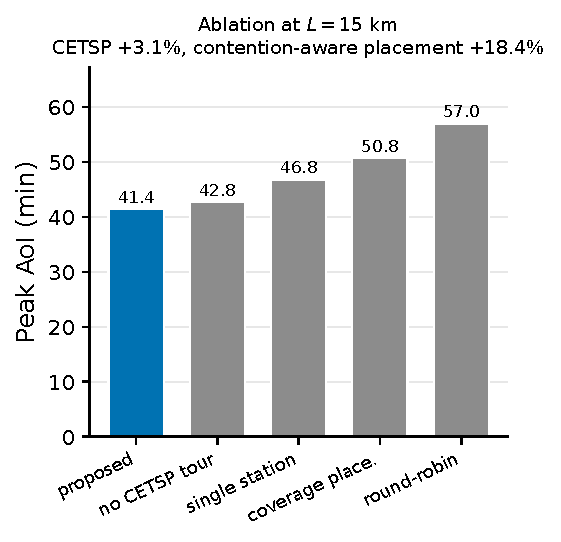
\includegraphics[width=0.92\columnwidth]{../results/fig_ablation.png}
  \caption{Ablation at a $15$~km field. Both the contention-aware placement and
  the CETSP trajectory contribute to the peak-AoI reduction of the proposed
  method.}
  \label{fig:ablation}
\end{figure}

Fig.~\ref{fig:crossover} sweeps the field size. The proposed distributed,
contention-aware placement beats the single pooled station at every field size,
and the gain grows with the field (from $4.1\%$ at $5$~km to $12.6\%$ at
$20$~km) because travel cost dominates as the field grows. We stress an honest
point: an earlier version using the open $M/M/c$ queue produced a spurious
crossover in which the single pooled station appeared to win in small fields.
That artifact came from the open queue overpenalizing split stations. With the
DES-validated finite-source model, whose wait saturates rather than diverging,
the artifact disappears and the distributed placement is preferred throughout.

\begin{figure}[t]
  \centering
  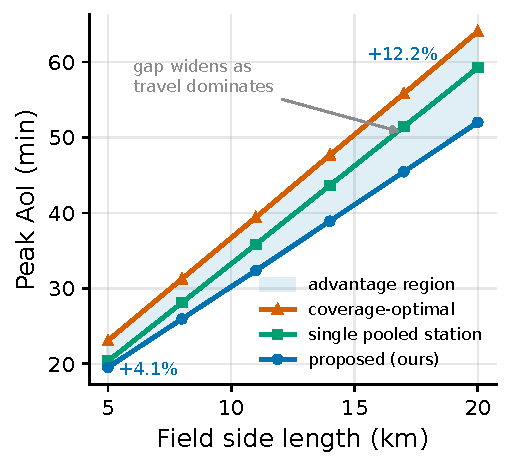
\includegraphics[width=\columnwidth]{../results/fig_crossover.png}
  \caption{Field-size sweep. The proposed distributed placement beats the single
  pooled station at all sizes, with a widening margin as travel cost grows.}
  \label{fig:crossover}
\end{figure}

\subsection{Discussion and design guidelines}
The results translate into concrete guidance for deploying a UAV swarm for fresh
data collection. First, the swarm should not be sized by coverage alone. Because
the peak AoI is non-monotone in the swarm size, there is a sweet spot
$M^\star$ beyond which extra UAVs only add charging congestion and worsen
freshness; Table~\ref{tab:mstar} shows that $M^\star$ is set by the installed
charging capacity, so the swarm size and the number of ports must be provisioned
together. When freshness targets tighten, adding ports (raising $M^\star$) is
often more effective than adding UAVs to an already congested system.

Second, charging stations should be placed to balance the queueing load, not
only to minimize flight detour. The coverage-optimal placement concentrates the
recharge traffic and inflates the wait; spreading the stations lowers the peak
AoI even at the cost of longer trips, and the benefit grows with the field size
because travel then dominates. A single pooled station remains a sensible choice
only in small fields where travel is cheap, which the field-size sweep makes
explicit.

Third, the queueing model matters as much as the optimizer. Treating the
charging system as an open $M/M/c$ queue overstates the wait by about $6\times$
and, as shown above, can flip a design decision (the spurious small-field
crossover). The finite-source model removes this bias and, being a conservative
upper bound on the near-deterministic reality, yields safe rather than
optimistic AoI estimates. We therefore recommend the finite-source model as the
default planning tool for swarm recharging with a bounded number of vehicles.

Finally, the ablation isolates where the gain comes from. The contention-aware
placement provides the larger share, while the GPU close-enough-TSP trajectory
adds a smaller but consistent improvement by shortening the revisit period at a
realistic collection radius. Both components are complementary, and the joint
solver combines them without violating the energy and budget constraints.
